\chapter{数値実験}
\label{chap:experiment}

本章では,提案したアルゴリズムの有効性を検証するための実験を行う.
実験で比較するアルゴリズムは次の通り.
\begin{enumerate}
\item Brandesのアルゴリズム(再計算)
  \par 辺が挿入または削除される度にBrandesのアルゴリズム(アルゴリズム\ref{algo:brandes})で媒介中心性を再計算する
\item 提案手法(更新)
  \par 辺が挿入された場合アルゴリズム\ref{algo:incremental-algorithm}で,削除された場合アルゴリズム\ref{algo:decremental-algorithm}で媒介中心性を更新する
\end{enumerate}

まず,人工ネットワークに対する実験を行う.具体的には,両アルゴリズムの実行時間の
比較を行う.また,提案手法について,更新したペア依存度の数と実行時間の関係および
媒介中心性を更新した頂点数と実際に媒介中心性が変化した頂点数の関係を明らかにすることで,
\ref{subsect:computational-complexity-of-incremental-algorithm}と
\ref{subsect:computational-complexity-of-decremental-algorithm}で
行った理論的な解析にさらなる根拠を与える.

次に,実ネットワークに対する実験を行う.実ネットワークに対する両アルゴリズムの実行時間の
比較を行う.さらに,実用上の観点から,頑健な道路ネットワークの構築と,
媒介中心性のリアルタイム計算への応用を想定した実験を行う.

なお,すべての実験は Intel (R) Xeon (R) CPU E-2620 v4 , 64GB RAM 上で行われた.
実験に用いたプログラムは gcc 7.2.0 によって, -O3 最適化フラグを付与してコンパイルされた.
プログラムのソースコードは\url{https://github.com/y-satotani/dynamic-betweenness}
にて入手可能である.

\section{人工ネットワークに対する実験}
\label{sect:exp-artificial}

本節では,以下の項目について実験を行い,その結果について考察する.
\begin{enumerate}
\item 両アルゴリズムの実行時間の比較
\item ペア依存度を更新した頂点ペアの数と実行時間の関係
\item 媒介中心性が実際に変化した頂点の数と更新した頂点の数の関係
\end{enumerate}

人工ネットワークとして次の二種類のネットワークモデルを用いる.
\begin{enumerate}
\item Erd\H{o}s--R\'{e}nyiモデル\cite{Erdos1959}
\item Barab\'{a}si--Albertモデル\cite{Barabasi1999}
\end{enumerate}

\subsection{両アルゴリズムの実行時間の比較}
この実験ではBrandesのアルゴリズムと提案手法の実行時間を比較する.
ネットワークの平均次数は$4$,頂点数は$100,200,\ldots,1000$とした.
それぞれのネットワークモデルのネットワークを100個生成して実験を行った.

図\ref{fig:exp-artificial-order}は各アルゴリズムの実行時間を比較したものである.
各ネットワークの平均次数はおよそ$4$である.それぞれの頂点数について,
100個のネットワークに対する実行時間の最大値および平均値を計算している.

\begin{figure}[tb]
  \centering
  \includegraphics{exp-artificial-order.pdf}
  \caption{頂点数に対する実行時間の比較}
  \label{fig:exp-artificial-order}
\end{figure}

図\ref{fig:exp-artificial-order}より,二種類のネットワークモデル両方に対して,
頂点数が増加するとともに更新の平均実行時間が再計算のものと比べて短くなっていることが分かる.
理由として,依存度を再計算する必要がある頂点が頂点数の増加とともに比較的少なくなることが考えられる.

\subsection{更新の量と実行時間の関係}

提案したアルゴリズムのようなオンラインアルゴリズムの性能を評価するためには,
アルゴリズムによって更新した要素の数を考慮する必要がある
\cite{Ramalingam1996,Lee2012,Pontecorvi2014}.
この実験によって,依存度を更新した頂点ペア数と実行時間の関係を明らかにする.さらに,
\ref{subsect:computational-complexity-of-incremental-algorithm}と
\ref{subsect:computational-complexity-of-decremental-algorithm}で
行った理論的な解析結果と,実験データが矛盾しないかを検証する.

依存度$\delta_{s\bullet}(v)$を更新した頂点ペア$(s,v)$を計数し,全体の更新に要した時間を計測した.
頂点数を$1000$,平均次数は$4$または$64$とし,$100$個のネットワークに対して更新を行った.

\begin{figure}[tb]
  \centering
  \includegraphics{exp-artificial-update.pdf}
  \caption{更新した頂点ペアの数に対する実行時間}
  \label{fig:exp-artificial-update}
\end{figure}

図\ref{fig:exp-artificial-update}は依存度を更新した頂点ペア数と実行時間の関係を表す.
図\ref{fig:exp-artificial-update}より,更新した頂点ペア数が少ないと,実行時間が短くなることが分かる.
さらに,次数が大きいと実行時間が長くなる.つまり,この性質は辺の数が増加すると実行時間も
増加することを示している.
また,この結果は理論的な解析結果と矛盾しない.

\subsection{媒介中心性を更新した頂点の数と変化した頂点の数の関係}
\ref{subsect:computational-complexity-of-incremental-algorithm}と
\ref{subsect:computational-complexity-of-decremental-algorithm}で
理論解析では,媒介中心性を更新した頂点の数と実際に媒介中心性が変化した頂点の数との
具体的な関係が不明なままであった.そのため,この実験によってその関係を明らかにする.

実際に媒介中心性が変化した頂点の数と,依存度$\delta_{s\bullet}(v)$を更新したような$s$が
存在する頂点$v$の数を計数する実験を行った.
両ネットワークモデルにおいて,頂点数を$1000$,平均次数を$4$として実験した.

\begin{figure}[tb]
  \centering
  \includegraphics{exp-artificial-phony.pdf}
  \caption{媒介中心性が変化した頂点数に対する,更新した頂点の数}
  \label{fig:exp-artificial-phony}
\end{figure}

図\ref{fig:exp-artificial-phony}に,媒介中心性を更新した頂点の数と
実際に媒介中心性が変化した頂点の数の関係を示す.
結果より,トポロジによって不要な更新の数が変化することがわかる.
特に,そのような更新はBarab\'{a}si--Albertモデルで顕著である.

\section{実ネットワークに対する実験}
\label{sect:exp-realnet}
前節の実験は人工的なネットワークの上のものであったが,
応用の観点から,実ネットワークに対するアルゴリズムの性能を知ることも重要である.
そこで,本節では実ネットワークに対する実験を行う.
まず,Stanford Large Network Dataset Collection\cite{Leskovec2016}から取得した実ネットワークでの性能評価を行い,
次に頑健な道路ネットワークの構築と,媒介中心性のリアルタイム計算への応用を想定した実験を行う.

\subsection{Stanford Large Network Dataset Collectionでの性能比較}
\label{subsect:exp-real}
Stanford Large Network Dataset Collectionのいくつかの実ネットワークに対して
両アルゴリズムの性能比較を行った.
両アルゴリズムを各ネットワークに対して10回実行し,その実行時間の平均値および最大値を求めた.
実験結果を表\ref{tab:exp-real}に示す.

\input{exp-misc.tex}

結果より,提案手法は実ネットワークでも高速に計算できることが確認できる.

\subsection{頑健な道路ネットワークの構築}
\label{subsect:exp-road}

第\ref{chap:introduction}章でも述べたように,道路ネットワークの頑健性を
向上するには,道路の建設によって媒介中心性の最大値を最小化する必要がある.
そこで,この実験では,実際の道路ネットワークに辺を挿入することによって,
媒介中心性の最大値を最小化させる.

道路ネットワークはOpenStreetMap\cite{OpenStreetMap}を利用して独自に構築した.
実験で用いる道路ネットワークを図\ref{fig:road-okayama}に示す.
このネットワークは$12165$個の頂点と$14820$本の辺を有する.

このネットワークに$9067$本の辺から一辺選んで追加したときの,媒介中心性が変化する様子を
調査する.同時に,$14820$本の辺から一辺選んで削除したときの様子も調査する.
なお,追加する辺について,図\ref{fig:road-okayama}において既にあるどの辺とも
交わらないような辺を選択した.

\begin{figure}[tb]
  \centering
  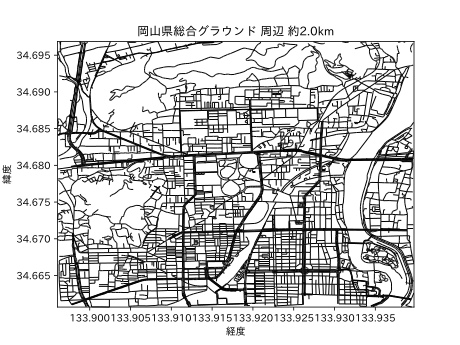
\includegraphics[width=.9\textwidth]{road-oka.eps}
  \caption{実験で用いる道路ネットワーク}
  \label{fig:road-okayama}
\end{figure}

図\ref{fig:exp-road-oka-correlation}は,一辺を挿入または削除したときの,
正規化された媒介中心性の最大値の分布である.
正規化された媒介中心性とは,媒介中心性を$2/\{(|V|-1)(|V|-2)\}$倍した値である.
辺の追加によって,最大$0.1607$の正規化された媒介中心性は$0.1379$まで減少し,
削除によって,$0.1225$まで減少させることに成功した.
また,辺追加によって媒介中心性の最大値が増加した例もある.
図\ref{fig:exp-road-oka-correlation}より,
媒介中心性が大きな頂点同士を結ぶと,媒介中心性の最大値が大きく変化することが分かる.

\begin{figure}[tb]
  \centering
  \includegraphics{exp-road-oka-correlation.eps}
  \caption{辺操作後の媒介中心性の最大値の分布}
  \label{fig:exp-road-oka-correlation}
\end{figure}

\subsection{媒介中心性のリアルタイム計算に関する実験}
\label{subsect:exp-sfhh}

第\ref{chap:introduction}章で説明したように,社会ネットワーク分析に
おいて,媒介中心性をはじめとした中心性に注目することは重要である.
しかし,現実の社会ネットワークでは,友人関係が時間とともに出現と消滅を繰り返している.
この実験では,友人関係の出現と消滅が頻繁に起こりうる状況で,
媒介中心性をリアルタイムで計算する用途への応用を想定する.

この実験では,SFHH conference data set\cite{Genois2018}というデータセットを用いた.
このデータセットは,2009にフランスで開催されたSFHHという会議の参加者$405$人に
赤外線タグを持たせて,参加者同士の交流の様子を時間とともに記録したものである.

図\ref{fig:exp-sfhh}は,データセットをもとにして辺の挿入と削除を
繰り返したときの各手法の実行時間を表す.あわせて,
20秒間のうちに発生した挿入と削除操作の回数の内訳を示す.

\begin{figure}[tb]
  \centering
  \includegraphics{exp-sfhh.pdf}
  \caption{SFHHに対する実験結果}
  \label{fig:exp-sfhh}
\end{figure}

図より,小規模な場合ではあるが,媒介中心性をリアルタイムに計算できる.
しかし,更新の量が多い場合,Brandesのアルゴリズムの方が高速に計算していることが分かる.
今後は,多くの辺の操作に対応するアルゴリズムの開発が課題である.
